\chapter{Problématique Réseau et SDN}
\label{chap-1}

%\section{Première section}\label{sec-1-1}

%\section{Deuxième section}\label{sec-1-2}

%Ce chapitre va reprendre les problèmes réseaux rencontrés pour définir les besoins actuels dans le domaine. Une liste de requis pour une architecture réseau idéalement adapté aux applications actuelles sera proposée.
%En connaissant les problèmes de l'architecture en place, la question que se pose est : si on repartait de zéro, comment on le ferrait ?

%\section{Pression pour l'expansion de l'architecture réseau }

\section{Ossification de l'internet face au besoin d'expansion}



%"The classic Internet architecture is a victim of its own success. Having succeeded so well at empowering users and encouraging innovation, it has been made obsolete by explosive growth in users, traffic, applications, and threats." The range of problems observed today is not surprising.

%The Internet was created in simpler times, among a small club of cooperating stakeholders. As the Internet becomes part of more and more aspects of society, it will inevitably be subject to more demands from more stakeholders, and be found deficient in more ways

%In the first half of the 2000s, the research climate was dominated by the belief that research is pointless unless its results can be adopted easily within the existing Internet. Attempting to work within this constraint, people realized that the current architecture makes solving some problems impossible.


À vouloir autoriser et même encourager les utilisateurs à innover sur son architecture, l'internet s'est fait dépasser par son propre succès. La croissance explosive des utilisateurs, du trafic et des applications a apporté toute une série de problèmes, 
%L'internet a été créé à une époque où les choses étaient plus simples, avec peu d'intervenants en coopération. Dès qu'il est devenu partie intégrante en plusieurs aspects de la société, diverses réclamations et défaillances sont apparues, 
tant que l'exhaustion des adresses IPv4 disponibles et les menaces aux réseaux locaux privés. 
\par
En réponse à ces questions, on a introduit dans l'architecture des \glspl{middlebox}, par exemple les NATs et les Firewalls, à un prix : la complexité. Le logiciel dans ces systèmes est capable d'atteindre n'importe quel objectif sous réserve de devenir excessivement complexe, fragile, incompréhensible et mal jugé. Parce que les coûts de la complexité ont été négligés lors de l'évolution de l'internet, les applications en réseau sortantes ont été rendues difficiles à concevoir, à mettre en place et à maintenir. \cite{InternetEvolutionRoleSoftwareEngineeringRealInternet}

Actuellement l'internet compte avec une énorme base d'équipements et de protocoles installée. Avec le système d'adressage IPv4 ce réseau peut interconnecter jusqu'à quatre milliards d'équipements. Capacité dont le limite est proche d'être atteint, confirmé par le développement du protocole IPv6 qui nous permettrait d'augmenter l'espace d'adressage par des centaines de milliards de fois. \cite{ICANNIPv6Important} 

L'internet est vu aujourd'hui comme une infrastructure critique de la société, tel que le transport ou l'électricité.  Cela provoque une résistance aux essais des nouvelles applications en parallèle à celles en mode de production. 
Ce fait a mené la communauté de chercheurs en réseau à se faire dominée par une conviction de qu'un travail n'est utile que si ses résultats peuvent être facilement adoptés dans l'architecture existante. En essayant de travailler avec cette contrainte, les concepteurs ont réalisé que l'architecture courante rend la résolution de certains problèmes impossible. \cite{OpenFlowStanfordOssification} \cite{SurveySDNIntro}

%illustrer les problèmes, donner un apperçu



%Complexity matters. The trouble with software is that it can do anything, no matter how complex, convoluted, fragile, incomprehensible, and ill-judged. Software engineers understand the cost of such complexity. Because the networking community underestimates the cost of complexity, it pays no attention to one of the most important problems of the current Internet, which is that it is much too difficult to build, deploy, and maintain networked applications.

%From the viewpoint of Internet users and application programmers, there are requirements that sometimes equal or exceed performance, availability, and efficiency in priority. These include ease of use, correctness, predictability, and modularity.

%The routing table in a typical router now has 300,000 entries, and these must be stored in the fastest, most expensive types of memory to maintain routing speed.

On se rend compte que l'adoption de nouvelles idées dans le domaine des réseaux reste complexe.  Finalement, les ingénieurs comptent avec peu de moyen concret pour tester de nouveaux protocoles réseau dans une configuration assez réaliste pour assurer et distribuer leurs déploiements. Par conséquent, la majorité des nouvelles idées émises dans le cadre de la recherche en "réseaux informatiques" finissent sans essais et sans tests. Cette barrière à l'évolution en face des besoins d'expansion des utilisateurs actuels confirme la croyance répandue que l'infrastructure réseau "est en phase d'ossification". \cite{OpenFlowStanfordOssification} 

%quantifier enorme.

\section{Management Réseau : Pénible et Complexe}

%\subsection*{Brain storming *}

%Même dans un réseau LAN de porte moyen,  on compte avec plusieurs équipements qui réalisent des fonctions spécifiques. Ces équipement doivent être configurable un à un donc pour atteindre à un objectif pour le réseau, tous la configuration de chaque équipement doit être orchestrée pour aboutir ce besoin. Il est difficile de mettre un place une configuration centralisée.

%\par Chaque équipement a été conçu pour réaliser une fonctionnalité spécifique. Pour toute correction de bug ou extension de ces fonctions,  il est nécessaire que le vendeur mette en place une mis à jour logiciel tenant en compte les modifications souhaités ou alors il faut acheter un nouveau équipement. 

%\par Difficulté de faire évoluer (lack of scalability or inability to scale) ; Complexité générant une résistance à l'innovation ; Dépendance du vendeur ; politiques inconsistantes

%Even with the help of autonomous and intelligent agents and network management software, the job of a network administrator is important and complicated. They must balance the different network management areas to make sure their system is properly configured and maintained. 

%The Internet was not designed with management in mind, yet the administrators of today’s networks face critical problems of configuration, traffic engineering, routing policy, and failure diagnosis. Their tools for understanding network traf- fic are poor, and their mechanisms for controlling network operations do not offer a predictable relationship between cause and effect.

%Internet routing is beginning to have serious problems of scale. The routing table in a typical router now has 300,000 entries, and these must be stored in the fastest, most expensive types of memory to maintain routing speed.2 There are efforts to move toward a scheme in which a typical routing table has one entry per autonomous system, which points to a router that can route to all the addresses for which that autonomous system is responsible.

%\subsection*{Fin brain storming *}

Cette résistance empêchant l'innovation est contradictoire à la rapide croissance de l'internet qui impose une expansion de l'architecture réseau. 
Le besoin pour des services réseau et débit augmente à un taux plus rapide que la disponibilité ou les revenues.



\begin{figure}[!h] %on ouvre l'environnement figure
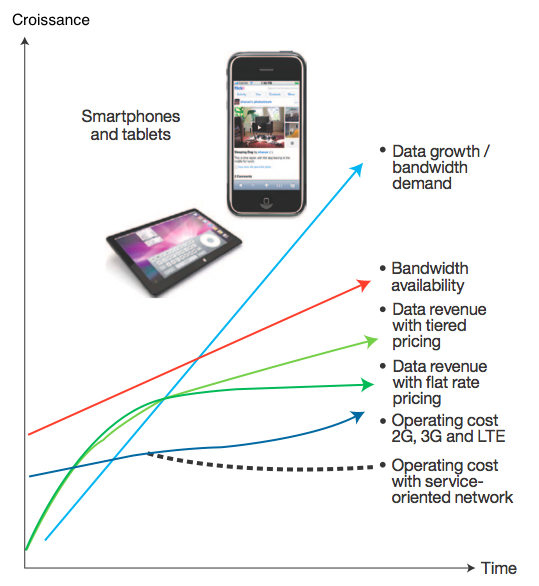
\includegraphics[width=15cm]{images/IncreasingPressureOnNetworkInfra.png} %ou image.png, .jpeg etc.
\caption{ Pression croissante sur l'infrastructure réseau \cite{IBMManagingGrowingPainsNeed}} %la légende
\label{image_soleil} %l'étiquette pour faire référence à cette image
\end{figure} %on ferme l'environnement figure


% Figure 1: The need for network capabilities and bandwidth is expanding at a faster rate than either bandwidth availability or revenue to grow

\clearpage

Le plus une entreprise dépend d'un nombre croissant de dispositifs et gros volumes de données, les plus importante est la demande pour débit et expansion de l'infrastructure. La complexité de cette expansion des réseaux augmente la probabilité des interruptions de service dues à une faille humaine ou autre problème. Ce fait met en évidence l'importance de la disponibilité, fiabilité, performance et sécurité. L'efficacité et la réduction des coûts deviennent cruciales pour aboutir la mis en échelle de ces besoins, et donc le management assume en rôle primordial dans ce contexte. \cite{IBMManagingGrowingPainsNeed}
 

Malgré l'assistance des agents autonomes et intelligents ainsi que des logiciels pour le management réseau, la mission de l'administrateur réseau reste importante et compliquée. Il doit équilibrer les différentes tâches du management pour assurer que le \gls{si} soit proprement configuré et maintenu. \cite{CentralIssuesNetworkManagementConclusion}



\section{Clean-slate Internet}

Re-partir de zéro. En le faisant, quels sont les caractéristique de l'architecture ?


Cette problématique a amené scientistes et les ingénieurs impliqués à concevoir \gls{sdn}. \gls{sdn} est un nouveau \glslink{paradigme}{paradigme} réseau qu'on fait actuellement en cours de développer pour adapter l'infrastructure existante au nouveau scénario.

\section{Les requis d'un réseau idéalement adapté aux besoins courants}